\chapter{Типы (или их отсутствие)}
\label{types-or-lack-thereof}
\section{Сильнейшая типизация}
Как вы, вероятно, заметили во время ввода примеров из \ref{starting-out-for-real}, а потом модулей и функций из \ref{modules}~и \ref{syntax-in-functions}, нам не нужно было вводить тип переменной или тип функции.
При сопоставлении с образцом нашему коду не нужно было знать, с чем производится сопоставление.
Кортеж \ops{\{X,Y\}} с одинаковым успехом можно сопоставить как с \ops{\{atom, 123\}}, так и с \ops{\{``A string'', <<``binary stuff!''>>\}}, \ops{\{2.0, [``strings'', ``and'', atoms]\}} или вообще с чем угодно.

При неудачном сопоставлении просто генерировалась ошибка, но она генерировалась только во время исполнения кода.
Причина этого \--- \emph{динамическая типизация} в языке Erlang.
Каждая ошибка ловится во время исполнения.
Если исполнение кода потенциально может закончиться аварией, то компилятор об этом не всегда будет истошно вопить, как в примере \ops{``llama + 5''} из главы \ref{starting-out-for-real}.

\begin{figure}[h!]
    \centering
    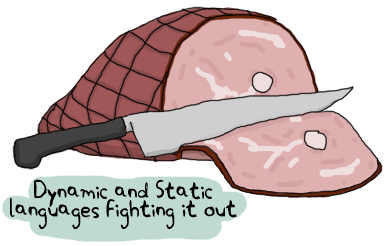
\includegraphics[width=0.4\textwidth]{ham.png}
\end{figure} 
Одной из классических точек трения между сторонниками статической и динамической типизации является безопасность програмного обеспечения.
Очень часто насаждается мысль, что хорошая статическая система типизации, за соблюдением которой с усердием следят компиляторы, будет ловить большинство ошибок ещё до того как код начнёт исполняться.
Поэтому языки со статической типизацией считаются более надёжными, чем их динамические собратья.
Хотя для многих динамических языков это действительно так, но к Erlang это относится не в полной мере, и его послужной список это подтверждает.
Лучшим примером служит степень готовности к обслуживанию (availability) \emph{девять девяток} (99.9999999\%), которая обеспечивается коммутаторами \href{http://www.erlang.se/publications/Ulf_Wiger.pdf}{Ericsson AXD 301 ATM}.
Количество строк Erlang\--кода для этих устройств \--- свыше 1 миллиона.
Обратите внимание \--- этот факт не свидетельствует о том, что ни один из компонентов системы, написанной на Erlang, не давал сбой.
Это означает, что коммутатор как единая система был готов к работе 99.9999999\% времени, включая запланированные перерывы.
Отчасти это заслуга проектировщиков, которые в разработке Erlang руководствовались идеей, что сбой в одной из компонент не должен влиять на всю систему.
При этом учитываются ошибки, которые допускает программист, сбои оборудования или сети.
Язык содержит средства, позволяющие распределять программы на различные узлы, обрабатывать непредвиденные ошибки и \emph{никогда} не останавливаться.

Иначе говоря, в то время как большинство языков и систем типизации стараются избавить программы от ошибок, Erlang использует стратегию, согласно которой считается, что ошибки будут возникать в любом случае, и старается эти случаи предотвратить.
Система динамической типизации в Erlang \--- не преграда для надёжности и безопасности программ.
Всё это очень напоминает речи проповедника, но в последующих главах вы увидите как это происходит.\\
\colorbox{lgray}
{
    \begin{minipage}{\linewidth}
\textbf{Замечание:} динамическая типизация в ретроспективе была избрана по простой причине.
Люди, которые занимались реализацией Erlang, в большинстве своём имели опыт программирования на языках с динамической типизацией, и поэтому динамическая типизация в Erlang была для них самым естественным выбором.
    \end{minipage}
}

Кроме того, Erlang \--- язык с сильной типизацией.
Языки со слабой типизацией производят неявные преобразования типов между термами.
Если бы Erlang был языком со слабой типизацией, то мы, вероятно, смогли бы исполнить операцию \ops{6 = 5 + ''1''}.
В действительности будет выброшено исключение, которое сообщает о неверных аргументах:
\begin{lstlisting}[style=erlang]
1> 6 + "1".
** exception error: bad argument in an arithmetic expression
    in operator  +/2
        called as 6 + "1"
\end{lstlisting}

Конечно же, есть случаи, когда вам хотелось бы преобразовать один вид данных в другой.
Например, привести обычный строковый тип к битовым строкам на время хранения, или целое значение привести к числу с плавающей запятой.
Для таких ситуаций Стандартная библиотека Erlang предлагает множество функций.
\section{Преобразование типов}
Как и многие языки, Erlang меняет тип терма посредством приведения его к другому типу.
Для этого применяются встроенные функции, поскольку многие преобразования невозможно реализовать на чистом Erlang.
Каждая такая функция имеет форму <тип>\_to\_<тип> и находится в модуле \ops{erlang}.
Вот некоторые из этих функций:
\begin{lstlisting}[style=erlang]
1> erlang:list_to_integer("54").
54
2> erlang:integer_to_list(54).
"54"
3> erlang:list_to_integer("54.32").
** exception error: bad argument
    in function  list_to_integer/1
        called as list_to_integer("54.32")
4> erlang:list_to_float("54.32").
54.32
5> erlang:atom_to_list(true).
"true"
6> erlang:list_to_bitstring("hi there").
<<"hi there">>
7> erlang:bitstring_to_list(<<"hi there">>).
"hi there"
\end{lstlisting}

И так далее.
Здесь мы сталкиваемся с неприятной особенностью языка.
Для именования функций используется схема <тип>\_to\_<тип>, поэтому при добавлении нового типа в язык приходится добавлять множество встроенных функций!
Вот их полный список:
\ops{atom\_to\_binary/2, atom\_to\_list/1, binary\_to\_atom/2}\\
\ops{binary\_to\_existing\_atom/2, binary\_to\_list/1,}\\
\ops{bitstring\_to\_list/1, binary\_to\_term/1, float\_to\_list/1,}\\
\ops{fun\_to\_list/1, integer\_to\_list/1, integer\_to\_list/2,}\\
\ops{iolist\_to\_binary/1, iolist\_to\_atom/1, list\_to\_atom/1,}\\
\ops{list\_to\_binary/1, list\_to\_bitstring/1,}\\
\ops{list\_to\_existing\_atom/1, list\_to\_float/1, list\_to\_integer/2,}\\
\ops{list\_to\_pid/1, list\_to\_tuple/1, pid\_to\_list/1,}\\
\ops{port\_to\_list/1, ref\_to\_list/1, term\_to\_binary/1,}\\
\ops{term\_to\_binary/2 и tuple\_to\_list/1.}

Многовато функций.
Большинство из них, если не все, мы увидим в этой книге.
Впрочем, все они нам вряд ли понадобятся.
\section{Охранять тип данных}
Базовые типы Erlang просто заметить: у кортежей есть фигурные скобки, у списков \--- квадратные, строки заключены в двойные кавычки и т.д.
Поэтому определённый тип данных можно использовать в сопоставлении с образцом: функция \ops{head/1}, которая принимает в качестве аргумента список, может принимать списки потому, что для других типов не сработало бы сопоставление (\ops{[H|\_]}).
\begin{figure}[h!]
    \centering
    
\includegraphics[width=0.3\textwidth]{my-name-is.png}
\end{figure} 

Тем не менее, у нас уже возникали проблемы с числовыми значениями, для которых мы не могли задавать диапазоны.
Для решения этой проблемы мы использовали стражи в функциях, которые были связаны с температурой, водительским возрастом и т.д.
Перед нами встаёт ещё одно препятствие.
Как нам записать страж, который применил бы сопоставление с образцом к данным лишь одного определённого типа, такого как числа, атомы или битовые строки?

Для решения этой задачи предназначены функции, которые возвращают истину, если переданный им аргумент имеет верный тип и ложь в противоположном случае.
Они составляют группу функций, которые допускаются в охранных выражениях и называются <<встроенными функциями проверки типов>>:
\begin{lstlisting}[style=erlang]
is_atom/1           is_binary/1        
is_bitstring/1      is_boolean/1        is_builtin/3       
is_float/1          is_function/1       is_function/2      
is_integer/1        is_list/1           is_number/1        
is_pid/1            is_port/1           is_record/2        
is_record/3         is_reference/1      is_tuple/1        
\end{lstlisting}

Их можно использовать, как и любое другое охранное выражение, в любом месте, где допускается охранное выражение.
Вы, вероятно, задаёте себе вопрос: почему функция просто не возвращает тип терма, который ей передали (что\--то вроде \ops{type\_of(X) -> Type}).
Ответ прост.
Erlang концентрируется на программировании для корректных ситуаций: вы составляете программу только для событий, которые точно должно произойти, для тех событий, которые вы ожидаете.
Всё прочее должно как можно раньше вызвать ошибку.
Может быть это покажется абсурдом, но объяснения, которые вы получите в главе \ref{errors-and-exceptions}, я надеюсь, прояснят ситуацию.
А пока что просто поверьте мне на слово.\\
\colorbox{lgray}
{
    \begin{minipage}{\linewidth}
\textbf{Замечание:} встроенные функции проверки типов более чем на половину состоят из инструкций, которые можно использовать в охранных выражениях.
Остальные функции также являются встроенными, но не относятся к функциям проверки типов.
Среди них: \ops{abs(Number), bit\_size(Bitstring), byte\_size(Bitstring),}
\ops{element(N, Tuple), float(Term), hd(List), length(List),}
\ops{node(), node(Pid|Ref|Port), round(Number), self(),}
\ops{size(Tuple|Bitstring), tl(List), trunc(Number), tuple\_size(Tuple).}\\
Функции \ops{node/1} и \ops{self/0} принадлежат к распределённым средствам Erlang и разделу процессов/акторов.
Вскоре мы будем их использовать, но до той поры мы ещё должны изучить много других вещей.
    \end{minipage}
}

Может показаться, что структуры данных в Erlang относительно ограничены, но списков и кортежей обычно достаточно для создания других более сложных структур.
Например, узел двоичного дерева можно представить как \ops{\{node, Value, Left, Right\}}, где \emph{Left} и \emph{Right} это или узлы, одинаковые по структуре, или пустые кортежи.
Я мог бы представить информацию о себе в таком виде:
\begin{lstlisting}[style=erlang]
{person, {name, <<"Fred T-H">>},
    {qualities, ["handsome", "smart", "honest", "objective"]},
    {faults, ["liar"]},
    {skills, ["programming", "bass guitar", "underwater breakdancing"]}}.
\end{lstlisting}

Этот пример показывает, как можно получить сложные структуры данных.
Для этого необходимо вложить списки в кортежи, заполнить их данными, и создать функции, которые будут работать с полученной структурой.\\
\colorbox{lgray}
{
    \begin{minipage}{\linewidth}
\textbf{Дополнение:}
в релизе R13B04 появилась встроенная функция \ops{binary\_to\_term/2}, которая позволяет десериализовать данные так же, как это делает \ops{binary\_to\_term/1}, с тем лишь отличием, что вторым аргументом можно передать список опций.
Если передать опцию \ops{[safe]}, то двоичные данные, содержащие неизвестные атомы или \ref{higher-order-functions}~анонимные функции, которые могут привести к исчерпанию памяти, декодированы не будут.
    \end{minipage}
}
\section{Для <<подсевших на систему>> типизации}
\label{for-type-junkies}
Этот раздел предназначен для программистов, которые по той или иной причине не представляют своё существование без статических систем типизации.
Он содержит слегка усложнённую теорию, которая не всем будет ясна.
Я кратко опишу инструменты, которые используются для статического анализа типов в Erlang, определения специализированных типов, и то, как всё это позволяет получить более безопасный код.
Эти средства будут описаны в книге намного позже, потому как они совсем не обязательны для разработки надёжных программ на Erlang.
Так как мы откладываем их рассмотрение на потом, я дам лишь основные сведения об их установке, запуске и т.д.
Повторюсь: этот раздел предназначен для тех, кто действительно не может жить без развитых систем типизации.
\begin{figure}[h!]
    \centering
    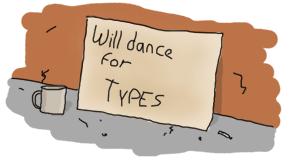
\includegraphics[width=0.4\textwidth]{type-dance.png}
\end{figure} 

На протяжении нескольких лет предпринимались попытки построения системы типов поверх Erlang.
Одна из таких попыток случилась в 1997 году под руководством Simon Marlow, одного из ведущих разработчиков Glasgow Haskell Compiler и Philip Wadler, который работал над проектированием Haskell и внёс свою лепту в теорию, которая лежит в основе монад (\href{http://www.haskell.org/~simonmar/papers/erltc.pdf}{вы можете прочитать документ} посвящённый упомянутой системе типов).
Joe Armstrong позже \href{http://www.cs.chalmers.se/Cs/Grundutb/Kurser/ppxt/HT2007/general/languages/armstrong-erlang\_history.pdf}{прокомментировал документ}:\\
\colorbox{lgray}
{
    \begin{minipage}{\linewidth}
Однажды мне позвонил Фил и заявил, что а) Erlang необходима система типов, б) он написал непольшой прототип такой системы и в) у него есть возможность взять творческий отпуск, в течение которого он собирался написать систему типов для Erlang, и спрашивал: <<будет ли нам это интересно?>>.
Я ответил: <<Да.>>\\
Phil Wadler и Simon Marlow работали над системой типов больше года, и результаты были опубликованы в [20].
Результаты оказались немного разочаровывающими.
Начнём с того, что на соответствие типов можно было проверять не весь язык, а лишь его подмножество.
Большим упущением было отсутствие типизированных процессов и отсутствие проверки типов для сообщений, пересылаемых между процессами.
    \end{minipage}
}

Процессы и сообщения относятся к основным средствам Erlang.
Может быть именно поэтому система так никогда и не была внедрена.
Были и другие неудачные попытки типизировать Erlang.
В результате усилий проекта HiPE (попытка увеличить производительность Erlang) появился Dialyzer, инструмент статического анализа, который используется до сих пор.
Он имеет свой собственный механизм вывода типов (type inference).

Система типов, которая в нём используется, основана на успешных типизациях (success typings) \--- концепции, которая отличается от системы типов Hindley\--Milner или мягкой типизации (soft\--typing).
Концепция успешной типизации проста: метод определение типов не пытается найти точный тип каждого выражения, но он гарантирует, что выведенные им типы точны, и что ошибки типов, которые он находит, действительно являются ошибками.

В качестве примера лучше всего привести реализацию функции \ops{and}, которая обычно принимает два булевых значения и возвращает 'true', если оба параметра истинны, иначе возвращается 'false'.
В системе типов Haskell это можно записать как \ops{and :: bool -> bool -> bool}.
Если бы нужно было реализовать функцию \ops{and} на Erlang, то это можно было бы сделать следующим образом:
\begin{lstlisting}[style=erlang]
and(false, _) -> false;
and(_, false) -> false;
and(true,true) -> true.
\end{lstlisting}

После применения метода успешной типизации, был бы выведен тип \ops{and(\_,\_) -> bool()}, где \_ означает 'любое значение'.
Причина этого проста: при вызыве функции с аргументами \ops{false} и \ops{42}, будет возвращён результат 'false'.
Использование шаблона подстановки \ops{\strut\_} в сопоставлении с образцом привело к тому, что для работы функции достаточно передать хотя бы один аргумент, который равен 'false'.
У системы типов ML случился бы припадок (а у её пользователей сердечный приступ), если бы вы вызвали функцию таким образом.
Но не у Erlang.
В этих строках появится больше смысла, если вы решите прочитать документ про \href{http://www.it.uu.se/research/group/hipe/papers/succ\_types.pdf}{реализацию успешной типизации}, в котором объясняется логика, которая стоит за таким поведением.
Я призываю каждого наркозависимого от типов прочитать эту статью.
Она представляет собой интересное и полезное описание реализации метода.

Подробности процесса определения типов и аннотирования функций описаны в Предложении об Улучшении Erlang №8 (\href{http://www.erlang.org/eeps/eep-0008.html}{EEP8}).
Если вас заинтересовало использование успешной типизации в Erlang, взгляните на \href{http://user.it.uu.se/~tobiasl/publications/typer.pdf}{приложение TypEr} и Dialyzer.
Оба входят в стандартный дистрибутив.
Чтобы ими воспользоваться, введите \ops{\$ typer --help} и \ops{\$ dialyzer --help} (для Windows команды \ops{typer.exe --help} и \ops{dialyzer --help}, если они доступны из текущей директории).

TypEr используется для аннотации типов функций.
Запуск TypEr для этой маленькой \href{http://learnyousomeerlang.com/static/erlang/fifo.erl}{реализации FIFO очереди} генерирует следующее описание типов:
\begin{lstlisting}[style=erlang]
%% File: fifo.erl
%% --------------
-spec new() -> {'fifo',[],[]}.
-spec push({'fifo',_,_},_) -> {'fifo',nonempty_maybe_improper_list(),_}.
-spec pop({'fifo',_,maybe_improper_list()}) -> {_,{'fifo',_,_}}.
-spec empty({'fifo',_,_}) -> bool().
\end{lstlisting}

Что, в целом, верно.
Improper списки лучше не использовать, так как с ними не работает функция \ops{lists:reverse/1}, а кто\--нибудь всё\--таки может попытаться протолкнуть такой список, минуя интерфейс модуля.
В этом случае функции \ops{push/2} и \ops{pop/2} всё\--таки отработают несколько вызовов, а затем будет выброшено исключение.
Поэтому нам необходимо добавить стражи, либо вручную оптимизировать определения типов.
Предположим, что мы добавили в модуль сигнатуру \ops{-spec push(\{fifo,list(),list()\},\_) -> \{fifo,nonempty\_list(),list()\}.} и функцию, которая передаёт improper список для \ops{push/2}.
При сканировании Dialyzer\--ом (который проверяет типы на соответствие), будет выведено сообщение об ошибке <<The call fifo:push({fifo,[1|2],[]},3) breaks the contract '<Type definition here>\'>>.
\begin{figure}[h!]
    \centering
    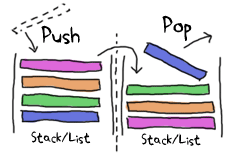
\includegraphics[width=0.4\textwidth]{fifo.png}
\end{figure} 

Dialyzer будет сообщать об ошибках лишь тогда, когда код будет нарушать работу другого кода, и эти сообщения, скорее всего, будут верными (он также будет сообщать и о других проблемах, например о ветках кода, до которых никогда не дойдёт исполнение или об общем рассогласовании).
При помощи Dialyzer\--а можно также анализировать полиморфные типы данных.
Функцию \ops{hd()} можно описать выражением \ops{-spec([A]) -> A.} и корректно проанализировать, впрочем программисты на Erlang редко используют этот синтаксис описания типов.\\
\colorbox{lorange}
{
    \begin{minipage}{\linewidth}
        \textbf{Не забывайтесь:}\\
Dialyzer и TypEr не обрабатывают классы типов с конструкторами, типы первого порядка и рекурсивные типы.
Типы в Erlang \--- это лишь аннотация, которая никак не влияет на компиляцию и не ограничивает её, кроме ситуаций, когда вы сами накладываете эти ограничения.
Программа проверки типов никогда не сообщит вам, что в приложении, которое работает прямо сейчас (или исполняется уже на протяжении двух лет), есть ошибка типов, которая никак себя не проявляет во время исполнения (корректное исполнение не говорит о том, что в коде нет ошибок\ldots)\\
Неплохо было бы иметь возможность создания рекурсивных типов, но они вряд ли когда\--нибудь появятся для TypEr и Dialyzer в текущем состоянии (объяснение можно найти в статье, указанной выше).
На текущий момент можно лишь вручную симулировать рекурсивные типы добавлением нескольких уровней вложенности.\\
Конечно же, это не нельзя назвать  всеобъемлющей системой типов, сравнимой со строгостью и мощью систем типизации в Scala, Haskell или OCaml.
Предупреждения и сообщения об ошибках обычно слегка запутаны и не всегда ясны пользователю.
Но если вы просто не можете существовать в мире динамического языка или жаждете дополнительной надёжности \--- это решение предлагает очень неплохой компромисс.
Относитесь к нему как к инструменту в вашем арсенале, не более.
    \end{minipage}
}
\colorbox{lgray}
{
    \begin{minipage}{\linewidth}
\textbf{Дополнение:}\\
Начиная с версии R13B04, в Dialyzer была добавлена экспериментальная возможность работы с рекурсивными типами.
Этот факт делает предыдущий раздел отчасти неверным.
Стыд мне и срам.\\
Также заметьте, что \href{http://erlang.org/doc/reference\_manual/typespec.html}{документация, описывающая типы, стала официальной} (хотя она и может в будущем измениться) и более полной, чем в EEP8.
    \end{minipage}
}
